\documentclass[xcolor=dvipsnames]{beamer}
\usecolortheme{whale}
\useoutertheme{infolines} % Alternatively: miniframes, infolines, split

\definecolor{UBCblue}{rgb}{0.04706, 0.13725, 0.26667} % UBC Blue (primary)
\definecolor{bostonuniversityred}{rgb}{0.8, 0.0, 0.0}

\usecolortheme[named=UBCblue]{structure}

\usepackage{wrapfig}
\pdfstringdefDisableCommands{%
  \def\\{}%
  \def\texttt#1{<#1>}%
}
\beamertemplatenavigationsymbolsempty


% Footnote
\setbeamertemplate{footline}{\leavevmode%
  \begin{beamercolorbox}[wd=.23\paperwidth,left,ht=2.5ex,dp=1.5ex,rightskip=4pt plus 1pt, leftskip=4pt]{subsection in head/foot}
    Manuel Paris
  \end{beamercolorbox}%
  \begin{beamercolorbox}[wd=.54\paperwidth,center,ht=2.5ex,dp=1.5ex]{section in head/foot}
    Sviluppo di uno Smart Contract IOTA
  \end{beamercolorbox}%
  \begin{beamercolorbox}[wd=.23\paperwidth,ht=2.5ex,dp=1.5ex,leftskip=4pt plus 1pt,rightskip=4pt plus 1pt]{subsection in head/foot}
    \hfill\insertframenumber/\inserttotalframenumber
  \end{beamercolorbox}%
}
\setbeamertemplate{section in toc}[sections numbered]
\setbeamertemplate{subsection in toc}[ball unnumbered]

\title{Sviluppo di uno Smart Contract IOTA}
\author{
  \texorpdfstring{\parbox{45mm}{\centering\scriptsize {\tiny Relatore:} \\ Prof. Dr. Marco Prandini }}{}
  \and
  \texorpdfstring{\parbox{45mm}{\centering\scriptsize {\tiny Correlatore:} \\ Dr. Giacomo Gori }}{} \and 
  \\[1em] \texorpdfstring{\parbox{45mm}{\centering\scriptsize {\tiny Presentato da:} \\ Manuel Paris }}{}
}
\institute{
  Corso di Laurea in Informatica\\
  Alma Mater Studiorum $\cdot$ Università di Bologna
}

\date{A.A. 2023-2024 \\ Sessione III}

\begin{document}
{
\setbeamertemplate{footline}{}
\begin{frame}
  \titlepage
\end{frame}
}
\addtocounter{framenumber}{-1}
%1
\begin{frame}{La rivoluzione di IOTA al settore delle blockchain}
    \linespread{1.5}
    \begin{itemize}
        \item Le \textbf{tecnologie di ledger distribuiti} sono affette da due principali problemi: la scarsa \textbf{scalabilità} della rete e la continua \textbf{inflazione} della moneta
        \vfill
        \item \textbf{IOTA Foundation} propone un nuovo sistema di ledger che punta a risolvere questi problemi
        \begin{itemize}
            \item Utilizza una struttura più complessa di una tradizionale blockchain, migliorando la scalabilità
            \item Elimina minatori di token e tasse sulle transazioni
        \end{itemize}
    \end{itemize}
\end{frame}

\begin{frame}{Il Tangle}
    \linespread{1.5}
    \begin{itemize}
        \item IOTA, al posto della struttura a catena delle blockchain, utilizza un grafo aciclico diretto, il \textbf{Tangle}
        \item Ogni nuova transazione ne approva due precedenti
    \end{itemize}
    \vfill
    \centering
    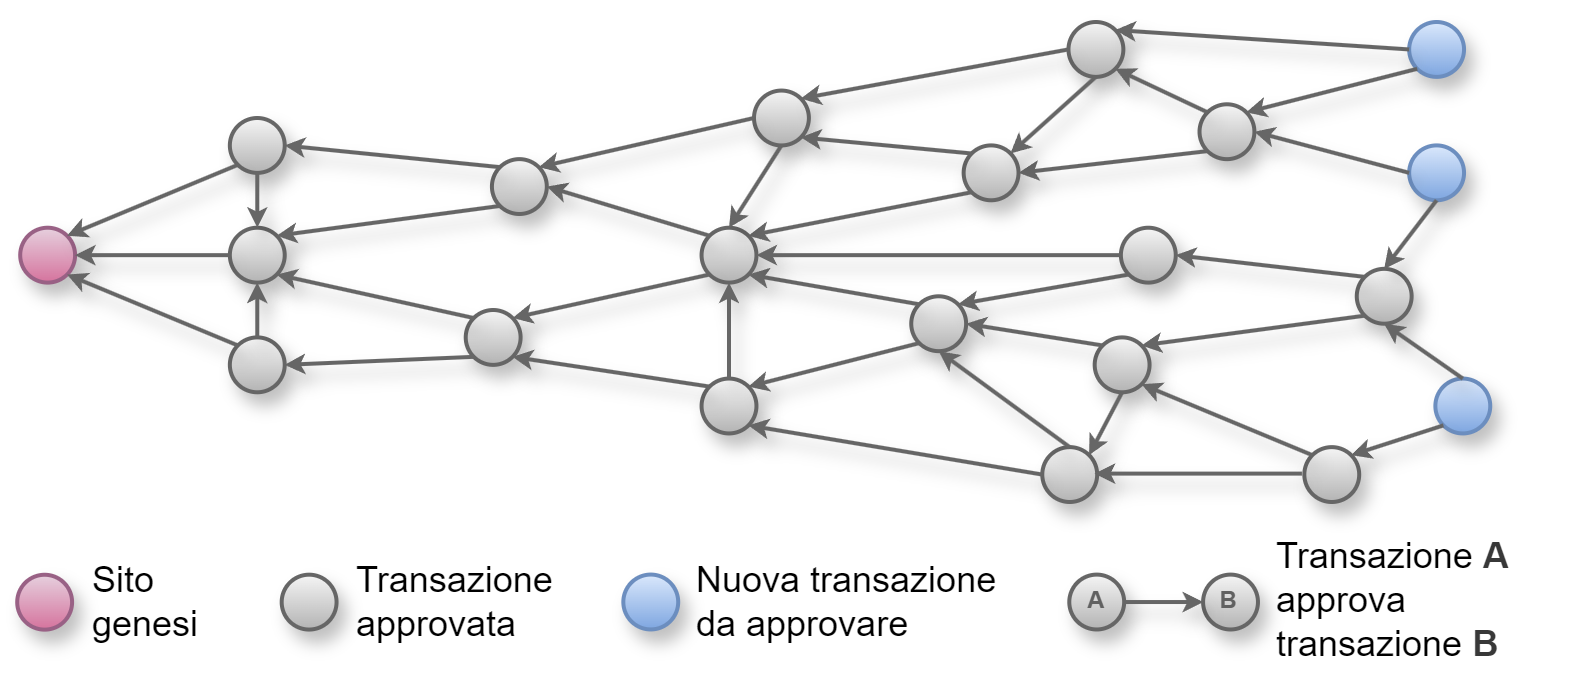
\includegraphics[width=0.8\textwidth]{figures/my_tangle.png}
\end{frame}

\begin{frame}{Come il Tangle risolve i problemi di scalabilità}
    \linespread{1.5}
    \begin{itemize}
        \item Le transazioni possono essere inserite anche contemporaneamente, invece che una alla volta
        \item In questo modo la grandezza della rete non influisce sulle prestazioni
    \end{itemize}
    \vfill
    \centering
    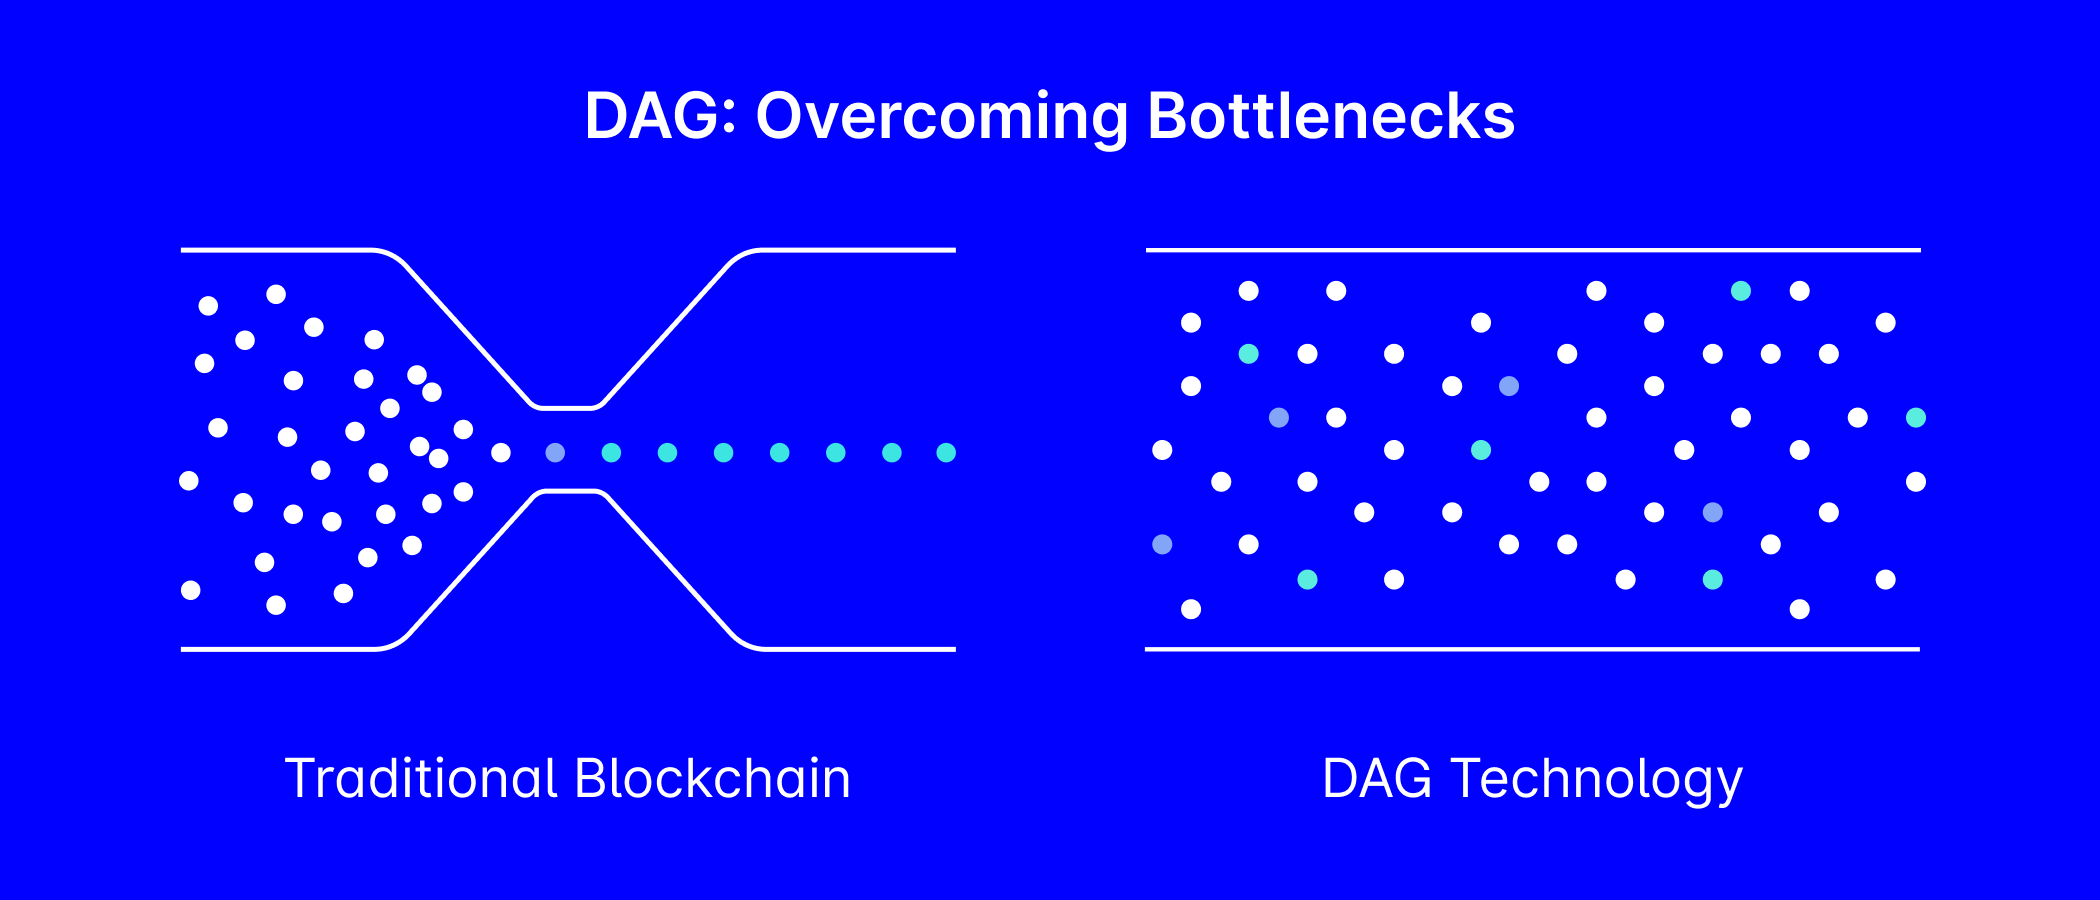
\includegraphics[width=0.7\textwidth]{figures/blockchain_bottleneck.png}
\end{frame}

\begin{frame}{Multi-ledger e Smart Contracts}
    \linespread{1.5}
    \begin{itemize}
        \item IOTA introduce un secondo ledger sopra al Tangle, formato da multiple blockchain
        \vfill
        \item Esse permettono di eseguire \textbf{Smart Contracts}, programmi che ampliano considerevolmente le possibilità di utilizzo del ledger
        \vfill
        \item Le chain agiscono in parallelo e possono comunicare fra di loro, fornendo \textbf{scalabilità} e \textbf{interoperabilità}
    \end{itemize}
\end{frame}

\begin{frame}{Smart Contract realizzato}
    \begin{columns}
        \begin{column}{0.5\textwidth}
            \centering
            Sistema di pagamenti\\[2em]
            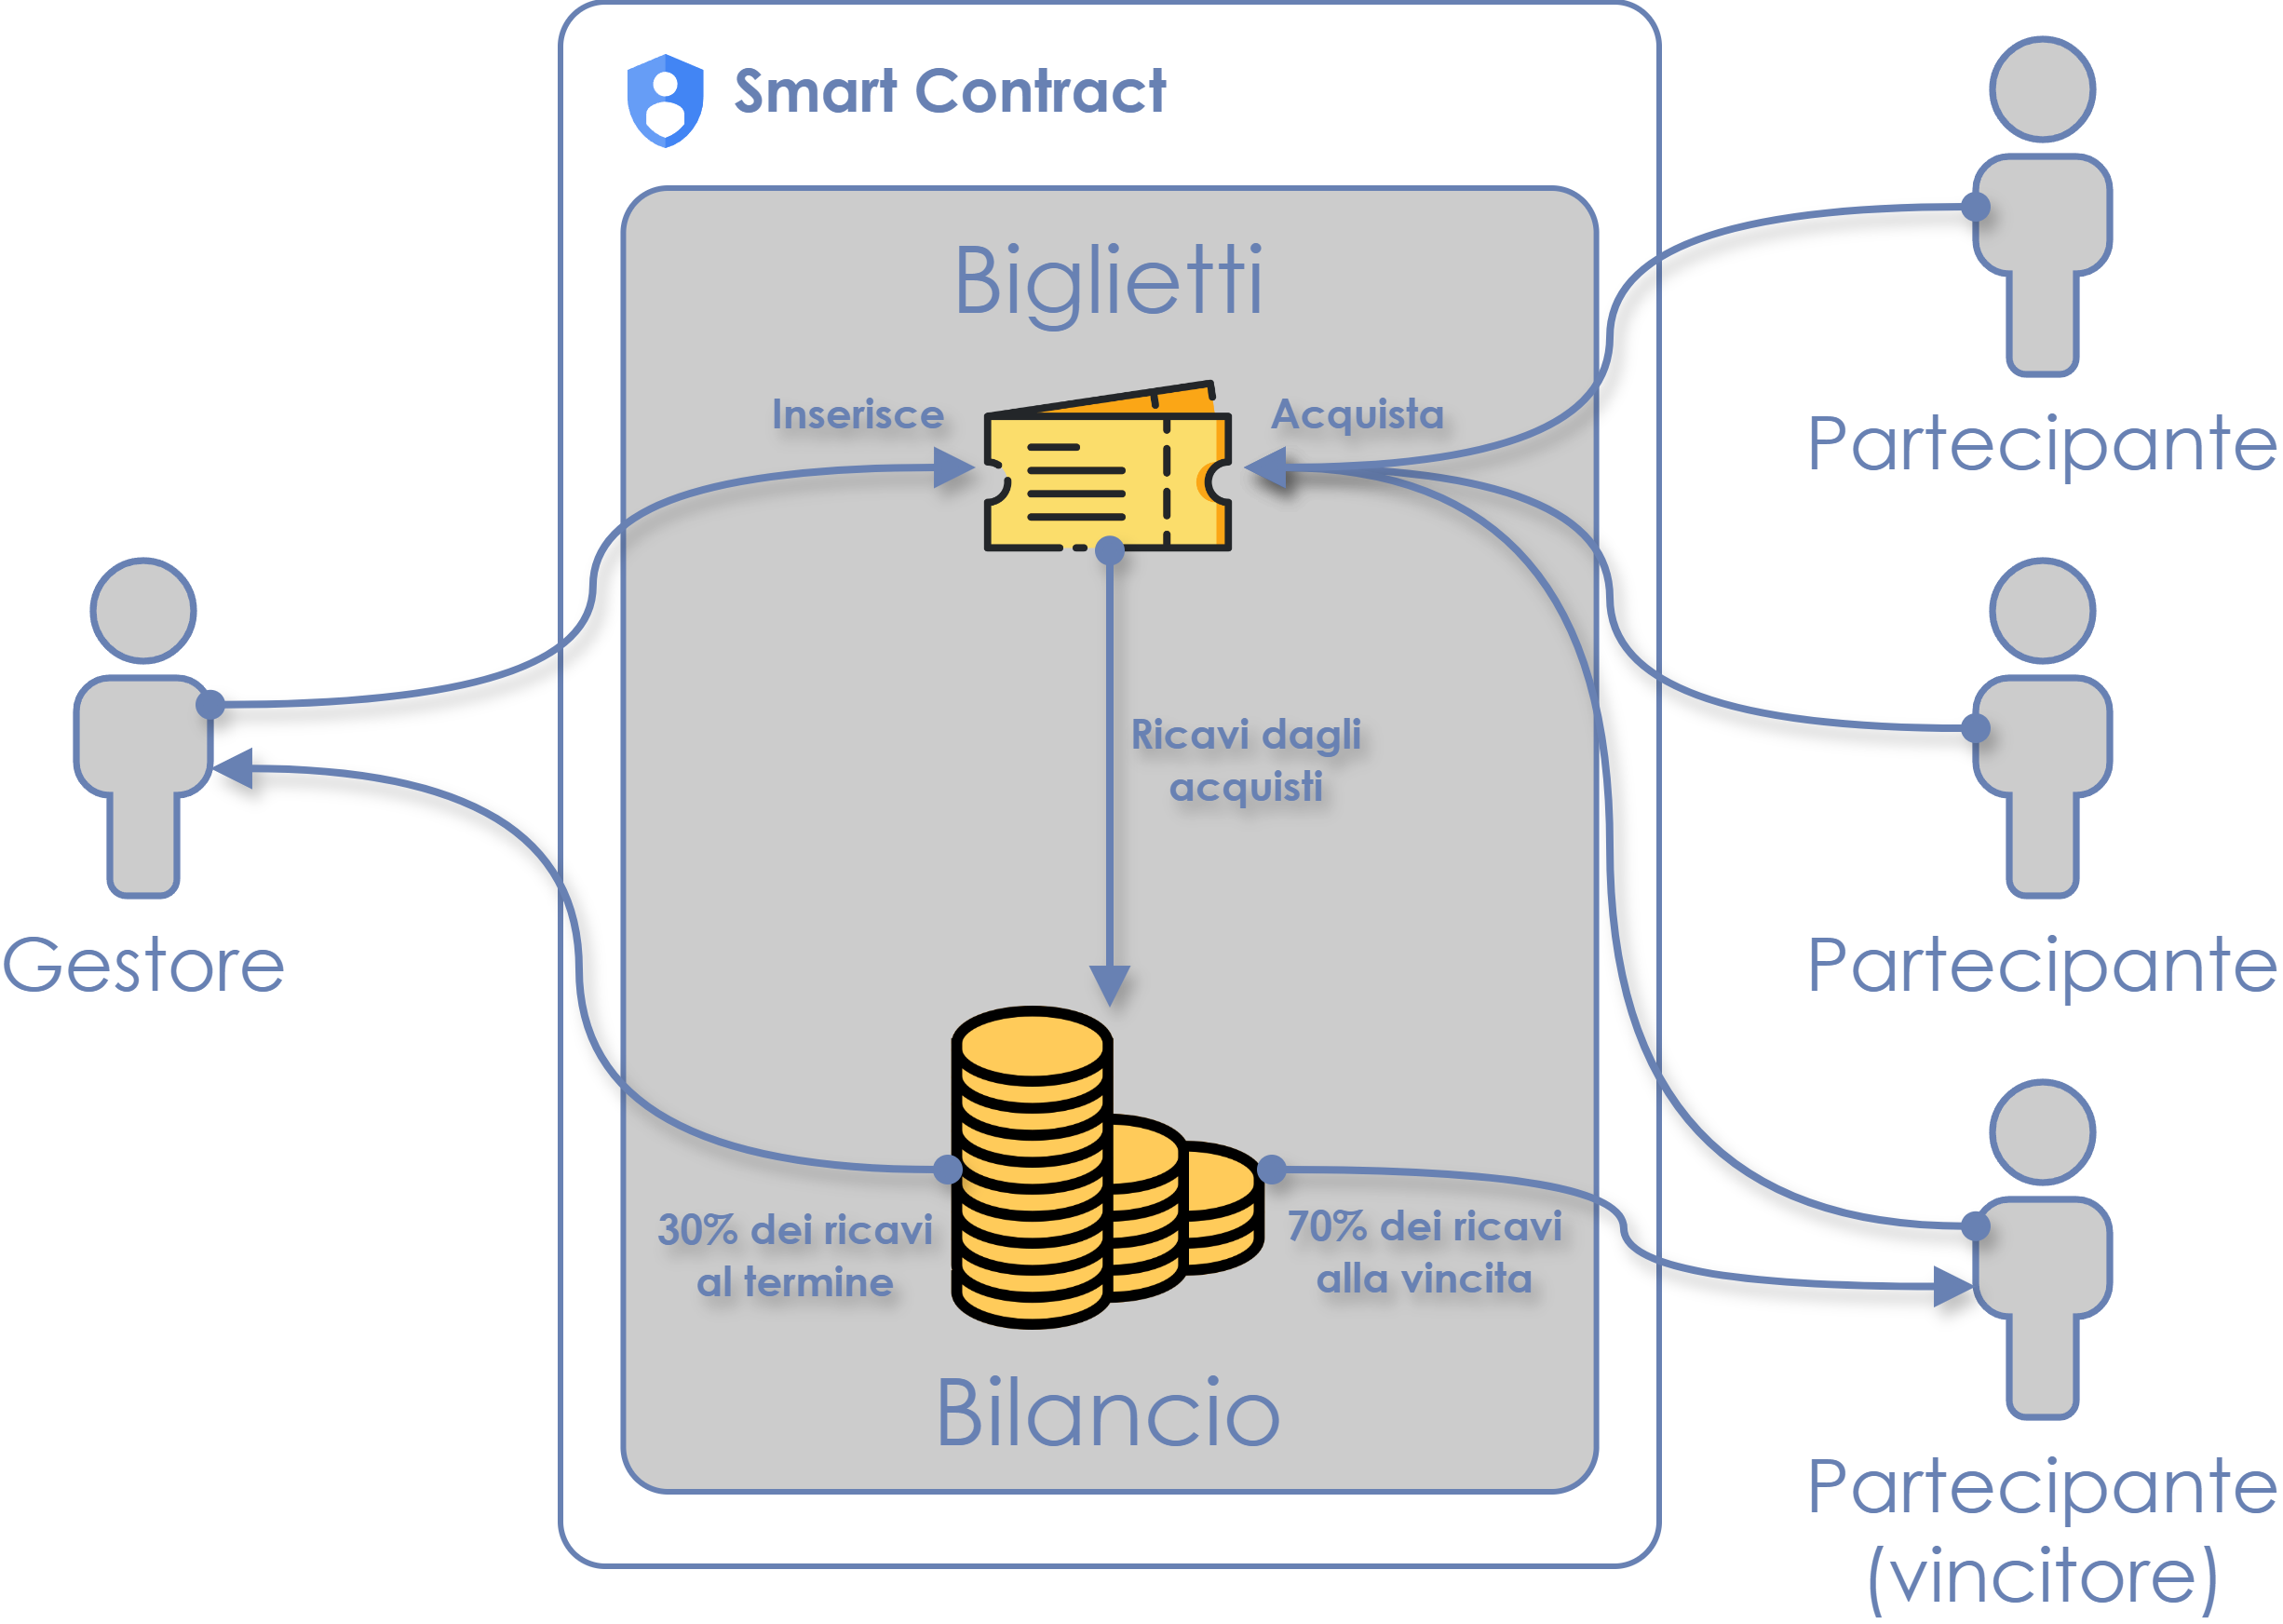
\includegraphics[width=\textwidth]{figures/my_app_diagram.png}
        \end{column}
        \begin{column}{0.5\textwidth}
            \centering
            Interazioni fra \textbf{WebApp} e \textbf{Smart Contract}\\[1em]
            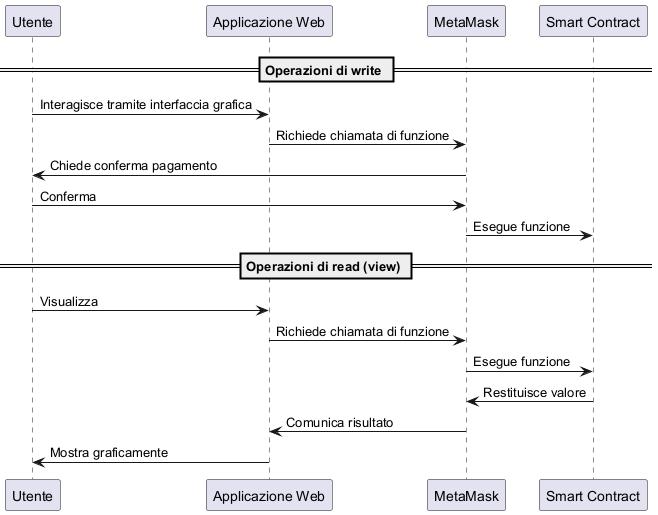
\includegraphics[width=\textwidth]{figures/my_interaction_diagram.png}
        \end{column}
    \end{columns}
\end{frame}

\begin{frame}{Analisi sulla programmazione in ledger distribuiti}
    \linespread{1.5}
    \begin{columns}
        \begin{column}{0.5\textwidth}
            \centering
            \color{teal}
            \textbf{\Large Vantaggi}
            {\setbeamercolor{item}{fg=teal}\begin{itemize}
                \item Massima \textbf{sicurezza} garantita
                \item Sistema di pagamenti \textbf{peer to peer} fornito dal ledger
                \item \textbf{Backend} per l'applicazione facilmente implementabile tramite \textbf{Smart Contract}
            \end{itemize}}
        \end{column}
        \begin{column}{0.5\textwidth}
            \centering
            \color{red}
            \textbf{\Large Limitazioni}
            {\setbeamercolor{item}{fg=red}\begin{itemize}
                \item \textbf{Tempi di esecuzione} più alti
                \item \textbf{Tasse} per interagire con Smart Contract 
                \item Necessario un account con dei fondi sul ledger, che ha una \textbf{user base} ancora ridotta
            \end{itemize}}
        \end{column}
    \end{columns}
\end{frame}

\begin{frame}{Prestazioni di IOTA}
    \begin{columns}
        \begin{column}{0.5\textwidth}
            \centering
            \large
            Operazioni \textbf{read}\\[1em]
            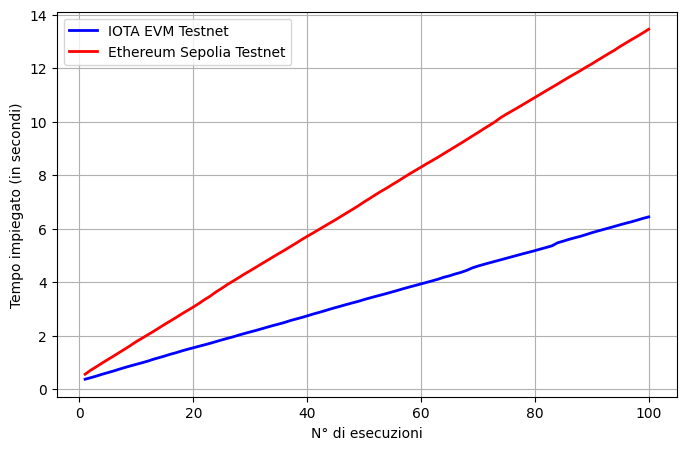
\includegraphics[width=\textwidth]{figures/my_is_lottery_open_runtime.png}
        \end{column}
        \begin{column}{0.5\textwidth}
            \centering
            \large 
            Operazioni \textbf{write}\\[1em]
            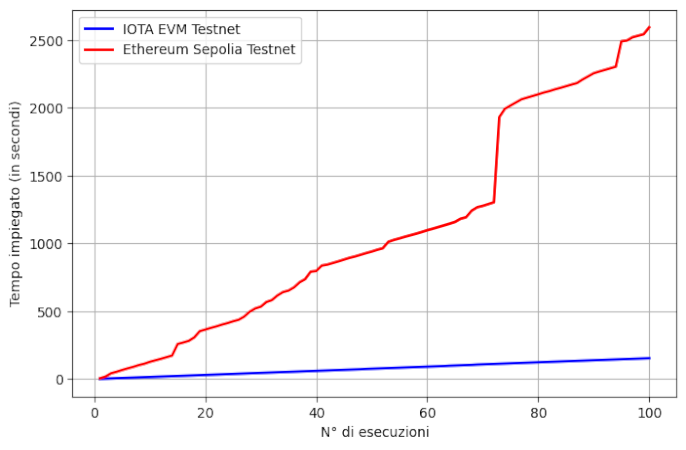
\includegraphics[width=\textwidth]{figures/my_buy_ticket_runtime.png}
        \end{column}
    \end{columns}
\end{frame}

\begin{frame}{Possibili sviluppi futuri}
    \linespread{1.5}
    \begin{itemize}
        \item Approfondire lo sviluppo di Smart Contract su IOTA, ampliandone gli ambiti applicativi e promuovendo l'efficienza di questo ledger
        \vfill
        \item Implementare sistemi di \textbf{tokenizzazione avanzata}, resa possibile dal ledger di IOTA
        \vfill
        \item Approcciarsi allo sviluppo sul nuovo \textbf{IOTA Rebased}, con il più avanzato linguaggio \textbf{Move} basato su risorse
    \end{itemize}
\end{frame}

\setbeamertemplate{footline}{} 
%13
\begin{frame}[noframenumbering]
    \centering \Large
    \emph{Grazie per l'attenzione}
\end{frame}
\end{document}